% Harus dimuat terlebih dahulu, digunakan agar file PDF memiliki format karakter yang benar.
% Untuk informasi lebih lanjut, lihat https://ctan.org/pkg/cmap.
\RequirePackage{cmap}

% Format dokumen sebagai paper konferensi menggunakan aturan IEEEtran terbaru (v1.8b).
% Untuk informasi lebih lanjut, lihat http://www.michaelshell.org/tex/ieeetran/.
\documentclass[conference]{IEEEtran}

% Format encoding font dan input menjadi 8-bit UTF-8.
\usepackage[T1]{fontenc}
\usepackage[utf8]{inputenc}
\usepackage{amsmath}
% Digunakan untuk mengatur margin dokumen.
\usepackage{textcomp}

% Digunakan untuk tujuan demonstrasi.
\usepackage{mwe}

% Digunakan untuk menampilkan font dengan style yang lebih baik.
\usepackage[zerostyle=b,scaled=.75]{newtxtt}

% Digunakan untuk menampilkan tabel dengan style yang lebih baik.
\usepackage{booktabs}
\usepackage[table,xcdraw]{xcolor}

% Digunakan untuk menampilkan gambar pada dokumen.
\usepackage{graphicx}

% Digunakan untuk menampilkan potongan kode.
\usepackage{listings}
\lstset{
  basicstyle=\ttfamily,
  columns=fixed,
  basewidth=.5em,
  xleftmargin=0.5cm,
  captionpos=b
}

\usepackage{tabularx}
\usepackage{wrapfig}
% Digunakan agar backticks (`) dapat dirender pada PDF.
% Untuk informasi lebih lanjut, lihat https://tex.stackexchange.com/a/341057/9075.
\usepackage{upquote}

% Digunakan untuk menyeimbangkan bagian akhir dokumen dengan dua kolom.
\usepackage{balance}

% Digunakan untuk menampilkan pustaka.
\usepackage[square,comma,numbers,sort&compress]{natbib}

% Mengubah format ukuran teks pada natbib.
\renewcommand{\bibfont}{\normalfont\footnotesize}

% Jika melebihi 3 penulis dapat dilakukan linebreakend 
\makeatletter
\newcommand{\linebreakand}{%
  \end{@IEEEauthorhalign}
  \hfill\mbox{}\par
  \mbox{}\hfill\begin{@IEEEauthorhalign}
}
\makeatother

% Menambah nama penulis ketika menggunakan perintah \citet.
% Untuk informasi lebih lanjut, lihat https://tex.stackexchange.com/a/76075/9075.
\usepackage{etoolbox}
\makeatletter
\patchcmd{\NAT@test}{\else \NAT@nm}{\else \NAT@hyper@{\NAT@nm}}{}{}
\makeatother

% Digunakan untuk melakukan linewrap pada pustaka dengan url yang panjang
% jika terdapat hyphens
\usepackage[hyphens]{url}

% Digunakan untuk menambah hyperlink pada referensi.
\usepackage{hyperref}

% Menonaktifkan warna dan bookmark pada hyperref.
\hypersetup{hidelinks,
  colorlinks=true,
  allcolors=black,
  pdfstartview=Fit,
  breaklinks=true
}

% Digunakan untuk membenarkan hyperref pada gambar.
\usepackage[all]{hypcap}

% Digunakan untuk menampilkan beberapa gambar
\usepackage[caption=false,font=footnotesize]{subfig}

\usepackage{stfloats}
% nama
\newcommand{\name}{Azzam Wildan Maulana}
\newcommand{\authorname}{Maulana, Azzam Wildan}
\newcommand{\nickname}{Wildan}
\newcommand{\advisor}{Muhtadin, S.T., M.T.}
\newcommand{\coadvisor}{Ahmad Zaini, S.T., M.T.}

% identitas
\newcommand{\nrp}{5024 20 1010}
\newcommand{\advisornip}{19800603 200604 1 003}
\newcommand{\coadvisornip}{19750419 200212 1 003}
\newcommand{\email}{5024201010@student.its.ac.id}
\newcommand{\advisoremail}{muhtadin@te.its.ac.id}
\newcommand{\coadvisoremail}{zaini@te.its.ac.id}

% judul
\newcommand{\tatitle}{KALIBRASI KAMERA \emph{OMNIVISION} PADA \emph{MOBILE ROBOT} MENGGUNAKAN \emph{MACHINE LEARNING}}
\newcommand{\engtatitle}{\emph{OMNIVISION CALIBRATION ON MOBILE ROBOT USING MACHINE LEARNING}}

% tempat
\newcommand{\place}{Surabaya}

% jurusan
\newcommand{\studyprogram}{Teknik Komputer}
\newcommand{\engstudyprogram}{Computer Engineering}

% fakultas
\newcommand{\faculty}{Teknologi Elektro dan Informatika Cerdas}
\newcommand{\engfaculty}{Intelligence Electrical and Informatics Technology}

% singkatan fakultas
\newcommand{\facultyshort}{FTEIC}
\newcommand{\engfacultyshort}{ELECTICS}

% departemen
\newcommand{\department}{Teknik Komputer}
\newcommand{\engdepartment}{Computer Engineering}

% Tambahkan format tanda hubung yang benar di sini
\hyphenation{
  ro-ket
  me-ngem-bang-kan
  per-hi-tu-ngan
}


\begin{document}

% Ubah kalimat berikut sesuai dengan judul penelitian.
\title{\engtatitle{}}

% Ubah kalimat-kalimat berikut sesuai dengan nama, institusi, alamat dan kontak penulis.
\author{
  \IEEEauthorblockN{1\textsuperscript{st} \name{}}
  \IEEEauthorblockA{\textit{dept. of \engstudyprogram{}}\\
    \textit{Institut Teknologi Sepuluh Nopember}\\
    Surabaya, Indonesia 60111\\
    \email{}}

  \and
  \IEEEauthorblockN{2\textsuperscript{nd} \advisor{}}
  \IEEEauthorblockA{\textit{dept. of \engstudyprogram{}}\\
    \textit{Institut Teknologi Sepuluh Nopember}\\
    Surabaya, Indonesia 60111\\
    \advisoremail{}}

  \and
  \IEEEauthorblockN{3\textsuperscript{rd} \coadvisor{}}
  \IEEEauthorblockA{\textit{dept. of \engstudyprogram{}}\\
    \textit{Institut Teknologi Sepuluh Nopember}\\
    Surabaya, Indonesia 60111\\
    \coadvisoremail{}}
}

% Digunakan untuk menampilkan judul dan deskripsi penulis.
\maketitle

% Mengubah keterangan `Abstract` ke bahasa indonesia.
% Hapus bagian ini untuk mengembalikan ke format awal.
% \renewcommand\abstractname{Abstrak}

\begin{abstract}

  % Ubah paragraf berikut sesuai dengan abstrak dari penelitian.
  \lipsum[1]


\end{abstract}

% Mengubah keterangan `Index terms` ke bahasa indonesia.
% Hapus bagian ini untuk mengembalikan ke format awal.
% \renewcommand\IEEEkeywordsname{Kata kunci}

\begin{IEEEkeywords}

  % Ubah kata-kata berikut sesuai dengan kata kunci dari penelitian.
  Deep Learning

\end{IEEEkeywords}


% Ubah bagian berikut sesuai dengan konten-konten yang akan dimasukkan pada dokumen
% Ubah judul dan label berikut sesuai dengan yang diinginkan.
\section{Introduction}
\label{sec:introduction}

% Ubah paragraf-paragraf pada bagian ini sesuai dengan yang diinginkan.
There are three main parts of Mobile Robot, namely Sensor, Control, and Actuator. All the main parts are connected to each other. Sensor is used to detect the environment around the robot. Control is used to process the data from the sensor and decide the next action. Actuator is used to execute the action that has been decided by the control.  
 
There is a sensor for Mobile Robot that can sense 360 degree around the robot. The sensor is called Omnivision Camera. The use of Omnivision Camera give more benefits because it can grab the information around robot with only one capture. The basic concept of Omnivision Camera is to use a mirror to reflect the environment around the robot. The mirror is placed in front of the camera. The camera is placed in the middle of the mirror and projected 90 degree to the ground of Robot. Not only can sense the environment around the robot, the camera can also sense within 10m distance. 

The hardware installation process of Omnivision Camera is hard. There are a common mistakes that everyone can accpet it such as misplaced camera, misplaced mirror, bad mirror, misplaced the whole system, and many more. Errors like that can cause a bad representation of the environment around the robot. The bad representation of the environment can cause the robot to make a wrong decision. 
% Ubah judul dan label berikut sesuai dengan yang diinginkan.
\section{Related Works}
\label{sec:relatedworks}

% Ubah paragraf-paragraf pada bagian ini sesuai dengan yang diinginkan.

Beberapa penelitian lain pernah dilakukan seperti yang dirumuskan oleh \citet{newton1687} bahwa \lipsum[5]
Hasil tersebut kemudian menjadi persamaan \ref{eq:hukumpertama}.

% Contoh pembuatan persamaan ilmiah.
\begin{equation}
  \label{eq:hukumpertama}
  \sum \mathbf{F} = 0\; \Leftrightarrow\; \frac{\mathrm{d} \mathbf{v} }{\mathrm{d}t} = 0.
\end{equation}

\lipsum[6-7]

\section{Design and Implementation}
\label{sec:desaindanimplementasi}

\subsection{System Description}
\label{sec:deskripsisistem}

\begin{figure}[ht]
  \centering
  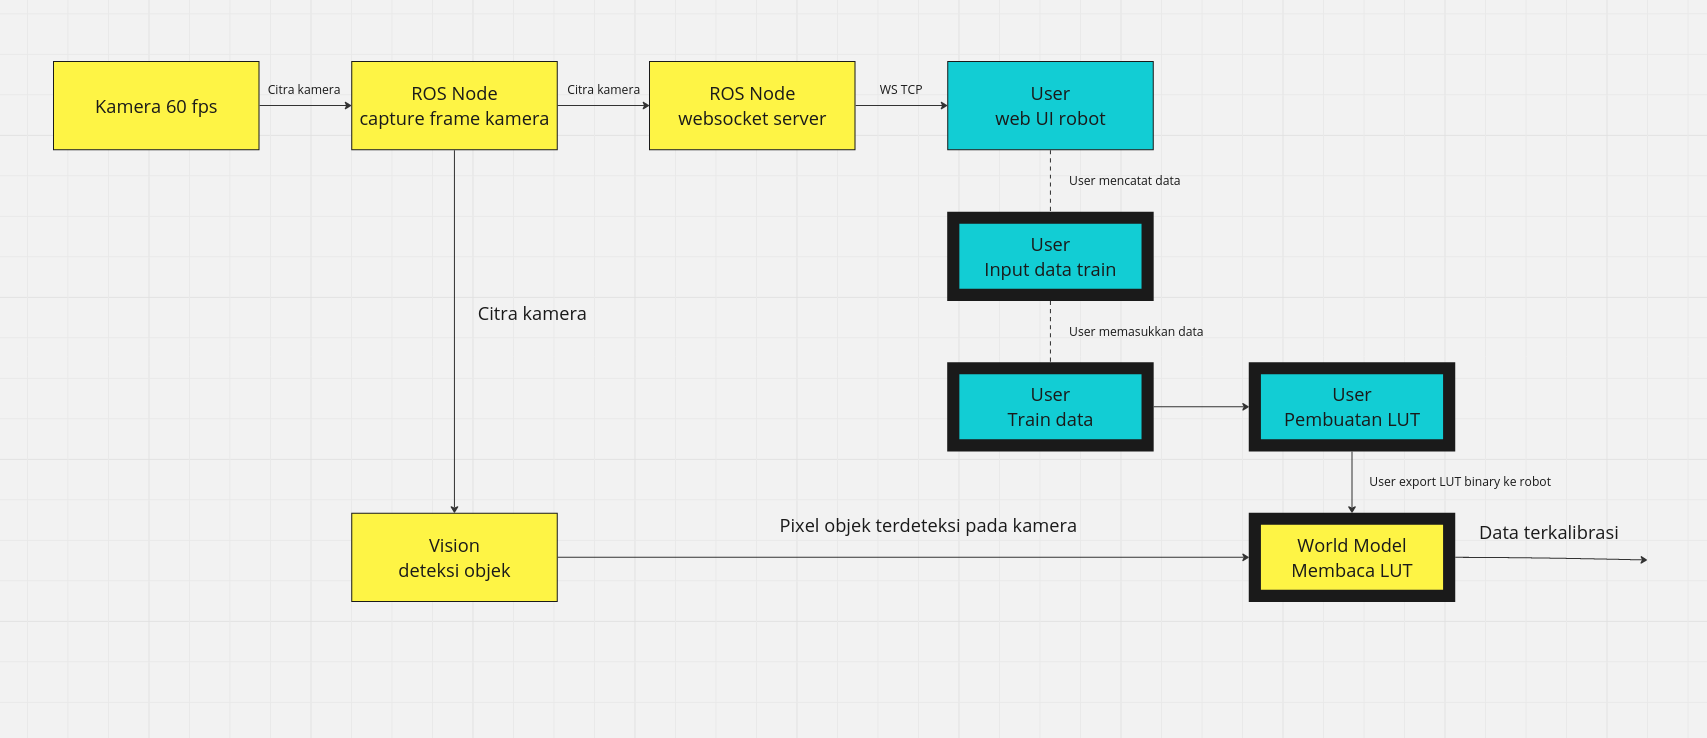
\includegraphics[width=8cm]{gambar/desain_sistem_vfix.png}
  \caption{Design System Block.}
  \label{fig:webrobot}
\end{figure}

From the figure above, the system is divided into two colors, namely yellow and cyan. The yellow color indicates that the process is running on the robot, while the cyan color indicates that the process is running outside the robot. The calibration system focuses on the system marked with a thick border, namely Data Retrieval, Data Training, Creating a Lookup Table, and the last is reading data from the Lookup Table so that it becomes calibrated data.

\subsection{Data Retrieval
  \label{sec:pengambilandata}}

The first thing to do before retrieving data is to prepare the robot and the marker that has been made before. The data taken is polar coordinate data both on the camera and on the field. The following formula is used to calculate polar coordinates on the camera:

\begin{equation}
  \begin{aligned}
    dx &= x - x\_center\_cam \\ 
    dy &= y\_center\_cam - y \\
    r &= \sqrt{dx^2 + dy^2} \\
    \theta &= \arctan(\frac{dy}{dx})
  \end{aligned}
\end{equation}

\begin{figure}[ht]
  \centering
  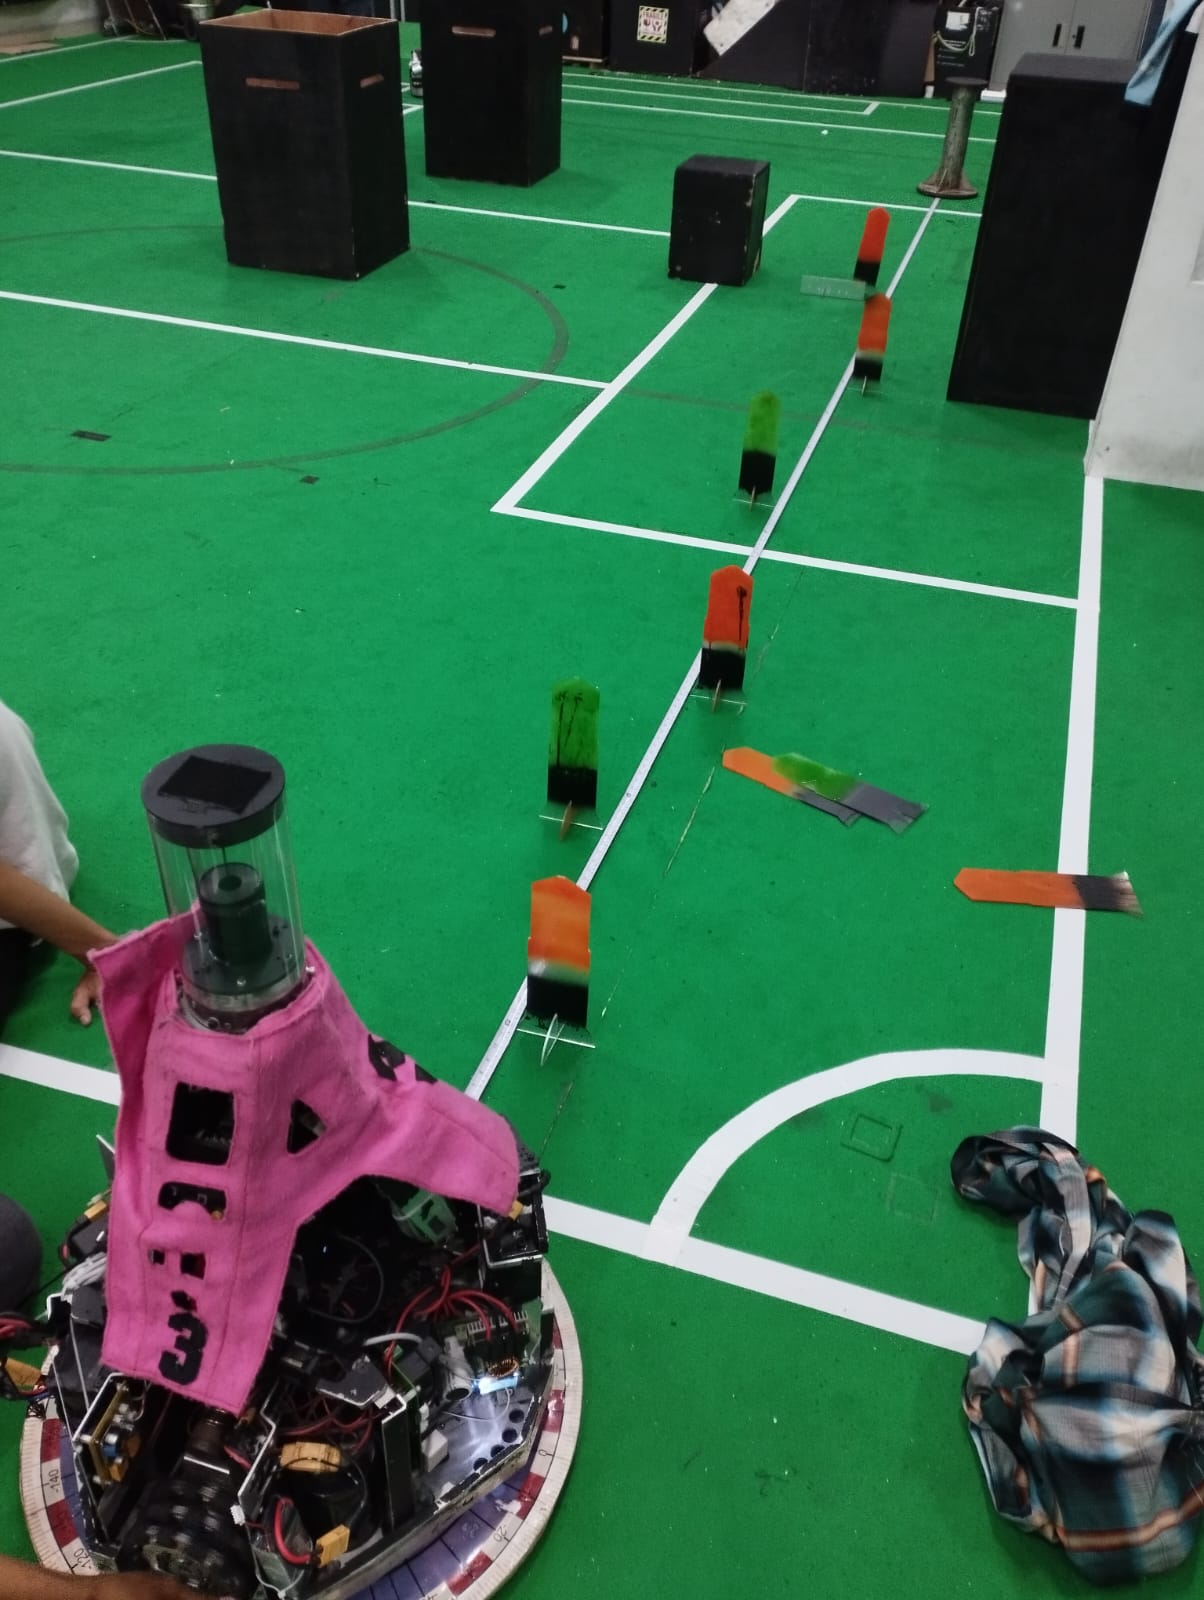
\includegraphics[width=5cm]{gambar/ambil_data.jpeg}
  \caption{Robot preparation.}
  \label{fig:persiapanrobot}
\end{figure}

Because the robot does not have a display, to access the camera needs to be done by accessing through the web program provided by the robot. The following is the view of robot camera displayed on the website.

\begin{figure}[ht]
  \centering
  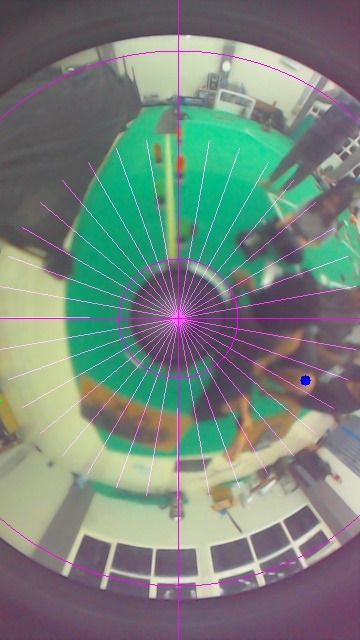
\includegraphics[width=5cm]{gambar/iris_web.jpeg}
  \caption{Robot camera display.}
  \label{fig:webrobot}
\end{figure}

From the website display, the red color on the field can be clicked and the polar coordinates on the camera will appear (according to the formula \textbf{3.1}). Then the coordinates will be saved to a file. The data taken is as follows:

\begin{table}[htbp]
  \caption{Training data.}
  \begin{center}
  \begin{tabular}{|c|c|c|}
    \hline
    \rowcolor[HTML]{C0C0C0}
    \textbf{Theta frame} & \textbf{Distance frame} & \textbf{Field distance} \\
    \hline
    0 deg            & 123.612 px                & 110 cm            \\
    0 deg           & 148.355 px                & 160 cm            \\
    0 deg           & 162.01 px                & 210 cm            \\
    0 deg           & 171.009 px                & 260 cm           \\
    10 deg           & 149.684 px                & 160 cm           \\
    19 deg           & 162.706 px                & 210 cm           \\
    10 deg           & 171.878 px                & 260 cm           \\
    20 deg           & 127.343 px                & 110 cm           \\
    20 deg           & 149.378 px                & 160 cm           \\
    20 deg           & 162.029 px                & 210 cm           \\
    20 deg           & 173.398 px                & 260 cm           \\
    ...           & ...                & ...           \\
    350 deg           & 147.681 px                & 160 cm           \\
    350 deg           & 159.797 px                & 210 cm           \\
    350 deg           & 169.577 px                & 260 cm           \\
    \hline
  \end{tabular}
  \label{tab1}
  \end{center}
\end{table}


\subsection{Training data
  \label{sec:trainingdata}}

The data that has been taken is then processed using the data training program. This program uses the Neural Network method to process the data. The following is the data training program.

The full architecture of the Neural Network used is having 2 hidden layers with 36 and 36 neurons each. The activation function used is Sigmoid with the formula as follows:

\begin{equation}
  \begin{aligned}
    f(x) &= \frac{1}{1 + e^{-x}}
  \end{aligned}
\end{equation}

The advantage of using Sigmoid is because Sigmoid has a value range between 0 and 1 which is suitable for the data to be processed.

The loss function used is the Mean Squared Error with the formula as follows:

\begin{equation}
  \begin{aligned}
    L(y, \hat{y}) &= \frac{1}{n} \sum_{i=1}^{n} (y_i - \hat{y_i})^2
  \end{aligned}
\end{equation}

The optimizer used is Adam with a learning rate of 0.0001.

The epoch used is 300000 times. It can change depending on the state of the data being trained.

The full architecture of the Neural Network used is as follows:

\begin{itemize}
    \item \( \mathbf{x} \in \mathbb{R}^2 \): Input data
    \item \( \mathbf{W}^{(1)} \in \mathbb{R}^{36 \times 2} \): weight layer 1
    \item \( \mathbf{b}^{(1)} \in \mathbb{R}^{36} \): bias layer 1
    \item \( \mathbf{W}^{(2)} \in \mathbb{R}^{36 \times 36} \): weight layer 2
    \item \( \mathbf{b}^{(2)} \in \mathbb{R}^{36} \): bias layer 2
    \item \( \mathbf{W}^{(3)} \in \mathbb{R}^{1 \times 36} \): weight layer 3
    \item \( \mathbf{b}^{(3)} \in \mathbb{R}^{1} \): bias layer 3
    \item \( \sigma \): sigmoid activation function
\end{itemize}

\begin{equation}
  \textbf{Input to Hidden Layer 1}:
  \begin{aligned}
    \mathbf{z}^{(1)} &= \mathbf{W}^{(1)} \mathbf{x} + \mathbf{b}^{(1)} \\
    \mathbf{a}^{(1)} &= \sigma(\mathbf{z}^{(1)})
  \end{aligned}
\end{equation}

\begin{equation}
  \textbf{Hidden Layer 1 to Hidden Layer 2}:
  \begin{aligned}
    \mathbf{z}^{(2)} &= \mathbf{W}^{(2)} \mathbf{a}^{(1)} + \mathbf{b}^{(2)} \\
    \mathbf{a}^{(2)} &= \sigma(\mathbf{z}^{(2)})
  \end{aligned}
\end{equation}

\begin{equation}
  \textbf{Hidden Layer 2 to Output Layer}:
  \begin{aligned}
    \mathbf{z}^{(3)} &= \mathbf{W}^{(3)} \mathbf{a}^{(2)} + \mathbf{b}^{(3)} \\
    \mathbf{a}^{(3)} &= \mathbf{z}^{(3)}
  \end{aligned}
\end{equation}

\subsection{Creating a Lookup Table
  \label{sec:pembuatanlut}}

After the data is trained, the data will be made into a Lookup Table. This Lookup Table contains the data that has been trained before. The following is the formula for creating a 2-dimensional Lookup Table:

\begin{equation}
  \begin{aligned}
    size &= \theta\_max \times r\_max \\
    index &= \theta \times r\_max + r
  \end{aligned}
\end{equation}

From the formula above, the size of the Lookup Table to be created and the index of the data to be entered into the Lookup Table can be obtained.
Then for the value of the Lookup Table itself comes from the formula \textbf{3.4 - 3.6}. These values will be entered into the Lookup Table according to the index calculated earlier.

\subsection{Reading the Lookup Table
  \label{sec:pembacaanlut}}

After the Lookup Table is created, the last thing is to read data from the Lookup Table with the formula as follows.

\begin{equation}
  \begin{aligned}
    index &= \theta\_cam \times r\_max + r\_cam \\
    r\_real &= \text{Lookup\_Table}[index] \\
    \theta\_real &= \theta\_cam
  \end{aligned}
\end{equation}

This process is done on the robot. The following is the Lookup Table reading program.






\section{Result and Discussion}
\label{sec:resultdiscussion}

\subsection{Calibration Result Visualization}
\label{sec:visualisasihasil}

The visualization of the calibration results is done by comparing the data on the camera with the data on the field. This is done by entering the camera data into the \emph{Lookup Table} that has been created before. The following is the visualization of the results obtained.

\begin{figure}[ht]
  \centering
  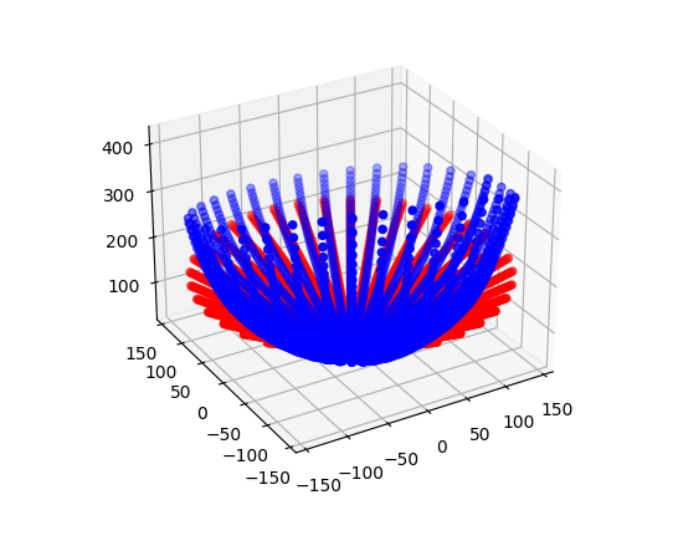
\includegraphics[width=5cm]{gambar/visual1.png}
  \caption{Visualization of calibration results.}
  \label{fig:hasilkalibrasi}
\end{figure}

From the figure above, it can be seen that the data on the camera used is not entirely projected perpendicular to the field. This happens because the camera used is not installed correctly.

\subsection{Accuracy Testing Scenario}
\label{sec:skenariopengujian}

The test is done by detecting a stationary ball on the field by rotating the robot in its position. This makes the robot able to see the ball from various angles. The test is done by taking data from the omnivision camera that has been installed on the robot and then processing the data using the \emph{Lookup Table} that has been created before so that the ball coordinates on the field are obtained. The following is the testing scenario that was carried out:

\begin{figure}[ht]
  \centering
  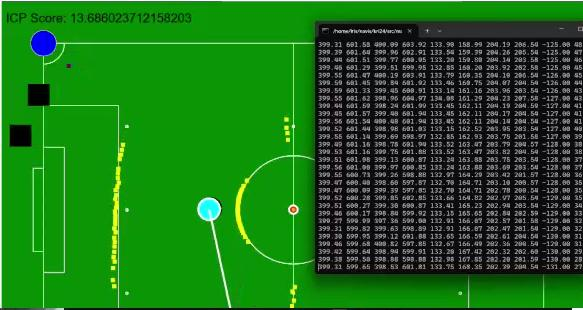
\includegraphics[width=8cm]{gambar/saat_putar_bola_2.jpeg}
  \caption{Testing Scenario.}
  \label{fig:skenariopengujian}
\end{figure}

The procedure is carried out at different distances between the robot and the ball on the field, namely at 120 cm, 200 cm, and 285 cm.

The formula used to calculate the ball's position on the field is as follows: 

\begin{equation}
  \begin{aligned}
    dx &= x\_ball\_cam - x\_center\_cam \\
    dy &= y\_center\_cam - y\_ball\_cam \\
    r\_ball\_cam &= \sqrt{dx^2 + dy^2} \\
    \theta\_ball\_cam &= \arctan(\frac{dy}{dx}) \\
    index &= \theta\_ball\_cam \times r\_max + r\_ball\_cam \\ 
    r\_ball\_fld &= r\_lookup[index] \\
    \theta\_ball\_fld &= \theta\_ball\_cam + robot\_\theta - 90 \\
    x\_ball &= robot\_x + r\_ball\_fld \times \cos(\theta\_ball\_fld) \\
    y\_ball &= robot\_y + r\_ball\_fld \times \sin(\theta\_ball\_fld) \\
  \end{aligned}
\end{equation}

\subsection{Accuracy Testing Evaluation}
\label{sec:analisispengujian}

While the test is running, the robot will rotate in its position to detect the ball on the field. The robot will rotate 30 degrees each time. The robot will rotate 12 times so that the robot can see the ball from all directions. After the robot has finished rotating, the robot will stop and the data will be recorded. The data obtained is the ball position on the field. The data is then compared with the actual ball position on the field. There are three tests that have been carried out, namely at a distance of 120 cm, 200 cm, and 285 cm. The following is the evaluation of the test results. The following data is obtained from the test results:

% Example of making a table

\begin{table}[htbp]
  \caption{Ball Position Test Results on the Field with a Distance of 120 cm.}
  \begin{center}
    \begin{tabular}{|c|c|c|}
      \hline
    \rowcolor[HTML]{C0C0C0}
  \textbf{Robot Angle to Ball} & \textbf{Ball Position X} & \textbf{Ball Position Y} \\
  \hline

  0 deg            & 407.74 cm                & 596.67 cm            \\
  30 deg           & 409.41 cm                & 600.3 cm            \\
  60 deg           & 409.65 cm                & 600.54 cm            \\
  90 deg           & 407.52 cm                & 598.2 cm           \\
  120 deg           & 407.18 cm                & 600.07 cm           \\
  150 deg           & 409.98 cm                & 598.35 cm           \\
  180 deg           & 410.66 cm                & 593.41 cm           \\
  210 deg           & 410.84 cm                & 590.28 cm           \\
  240 deg           & 410.01 cm                & 590.8 cm           \\
  270 deg           & 409.9 cm                & 594.28 cm           \\
  300 deg           & 408.91 cm                & 590.14 cm           \\
  330 deg           & 408.8 cm                & 591.57 cm           \\
  \hline
\end{tabular}
\end{center}
\end{table}

\begin{table}[htbp]
  \caption{Ball Position Test Results on the Field with a Distance of 200 cm.}
  \begin{center}

  \begin{tabular}{|c|c|c|}
  \hline
  \rowcolor[HTML]{C0C0C0}
  \textbf{Robot Angle to Ball} & \textbf{Ball Position X} & \textbf{Ball Position Y} \\
  \hline
  0 deg            & 406.44 cm                & 613.13 cm            \\
  30 deg           & 411.09 cm                & 624.66 cm            \\
  60 deg           & 416.39 cm                & 627.02 cm            \\
  90 deg           & 411.55 cm                & 625.85 cm           \\
  120 deg           & 408.85 cm                & 620.01 cm           \\
  150 deg           & 414.2 cm                & 611.7 cm           \\
  180 deg           & 415.12 cm                & 601.25 cm           \\
  210 deg           & 412.78 cm                & 592.09 cm           \\
  240 deg           & 410.77 cm                & 594.57 cm           \\
  270 deg           & 409.66 cm                & 598.43 cm           \\
  300 deg           & 407.92 cm                & 599.03 cm           \\
  330 deg           & 406.29 cm                & 602.72 cm           \\
  \hline
\end{tabular}
\end{center}
\end{table}

\begin{table}[htbp]
\caption{Ball Position Test Results on the Field with a Distance of 285 cm.}
\begin{center}

\begin{tabular}{|c|c|c|}
  \hline
  \rowcolor[HTML]{C0C0C0}
  \textbf{Robot Angle to Ball} & \textbf{Ball Position X} & \textbf{Ball Position Y} \\
  \hline
  0 deg            & 380.98 cm                & 593.81 cm            \\
  30 deg           & 382.14 cm                & 594.49 cm            \\
  60 deg           & 383.41 cm                & 607.18 cm            \\
  90 deg           & 392.49 cm                & 604.67 cm           \\
  120 deg           & 390.32 cm                & 606.04 cm           \\
  150 deg           & 391.43 cm                & 598.47 cm           \\
  180 deg           & 387.17 cm                & 587.89 cm           \\
  210 deg           & 390.16 cm                & 577.15 cm           \\
  240 deg           & 389.67 cm                & 585.82 cm           \\
  270 deg           & 389.38 cm                & 590.31 cm           \\
  300 deg           & 382.61 cm                & 593.25 cm           \\
  330 deg           & 380.73 cm                & 589.31 cm           \\
  \hline
\end{tabular}
\end{center}
\end{table}

Each table contains the ball position data on the field at different distances. Every data in that table is the ball position data on the field at a certain angle. The data is then compared with the actual ball position on the field. The comparison is done by calculating the standard deviation of the data obtained. The formula used to calculate the standard deviation is as follows: 

\begin{equation}
  \begin{aligned}
    \sigma &= \sqrt{\frac{\sum_{i=1}^{n} (x_i - \bar{x})^2}{n}} \\ 
  \end{aligned}
\end{equation}

Where $\sigma$ is the standard deviation, $x_i$ is the data, $\bar{x}$ is the average of the data, and $n$ is the number of data.

From the table, the standard deviation in the ball position data on the field with a distance of 120 cm is 1.26 cm and 4.11 cm for the ball position x and y. Meanwhile, at a distance of 200 cm, the standard deviation is 3.28 cm and 12.80 cm for the ball position x and y. At a distance of 285 cm, the standard deviation is 4.40 cm and 8.92 cm for the ball position x and y. 

From these results, it can be concluded that the calibration system that has been created can detect the ball position on the field well. The ball not being exactly in the middle of the field can be caused by several factors. Some of the factors causing this are the inaccuracy of the ball position in the real world, the inaccuracy of the robot position in the real world, and the inaccuracy of the robot orientation in the real world. Because basically according to the formula \textbf{4.1}, the ball position on the field is also determined by the robot's position on the field.

\subsection{Second Accuracy Testing Scenario}
\label{sec:skenariopengujian2}

The second accuracy test is by comparing the new calibration results with the old calibration that still uses the \emph{polynomial regression} algorithm. The test is done in the same way as the previous accuracy test. However, the calculation process uses the \emph{polynomial regression} algorithm.

\subsection{Second Accuracy Testing Evaluation}
\label{sec:analisispengujian2}

The test is done by comparing the data obtained from the new calibration with the data obtained from the old calibration. The following is the data obtained from the test results: 

\begin{table}[htbp]

\caption{Ball Position Test Results on the Field with a Distance of 120 cm using the Old Calibration.}
\begin{center}

\begin{tabular}{|c|c|c|}
  \hline
  \rowcolor[HTML]{C0C0C0}
  \textbf{Robot Angle to Ball} & \textbf{Ball Position X} & \textbf{Ball Position Y} \\
  \hline
  0 deg            & 370.18 cm                & 576.31 cm            \\
  30 deg           & 376.24 cm                & 585.42 cm            \\
  60 deg           & 383.91 cm                & 597.98 cm            \\
  90 deg           & 392.99 cm                & 605.67 cm           \\
  120 deg           & 390.23 cm                & 610.94 cm           \\
  150 deg           & 400.49 cm                & 598.89 cm           \\
  180 deg           & 385.97 cm                & 582.89 cm           \\
  210 deg           & 398.61 cm                & 577.15 cm           \\
  240 deg           & 390.76 cm                & 585.02 cm           \\
  270 deg           & 386.32 cm                & 588.91 cm           \\
  300 deg           & 378.69 cm                & 585.55 cm           \\
  330 deg           & 370.32 cm                & 579.11 cm           \\
  \hline
\end{tabular}
\end{center}
\end{table}

From the data, it can be seen that the standard deviation in the ball position data on the field with a distance of 120 cm using the old calibration is 10.01 cm and 11.32 cm for the ball position x and y. Meanwhile, in the new calibration, the standard deviation is 1.26 cm and 4.11 cm for the ball position x and y. It can be seen that the new calibration is better than the old calibration. This happens because the camera is not installed correctly on the robot, causing the old calibration results to be inaccurate. The inaccuracy occurs because the old calibration only uses one direction as a reference for the polynomial regression model. Whereas, in reality, the model formula for each camera direction will always be different.

\subsection{Third Accuracy Testing}
\label{sec:skenariopengujian3}

The third accuracy test is placing robot somewhere on the field and then the robot will see lines around the robot. The robot will detect each pixel of line and then the robot will calculate the distance between the robot and the line. So the robot can visualize the line on the field. The test is done by taking data from the omnivision camera that has been installed on the robot and then processing the data using the \emph{Lookup Table} that has been created before so that the line coordinates on the field are obtained. The following is the testing scenario that was carried out: 

\begin{figure}[htbp]
  \centering
  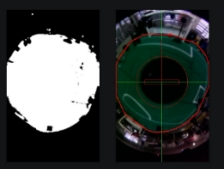
\includegraphics[width=7cm]{gambar/cam_raw1.jpg}
  \caption{Raw frame.}
  \label{fig:skenariopengujian31}
\end{figure}

The left picture is the field binary image that calculated to get the line binary image. 

\begin{figure}[htbp]
  \centering
  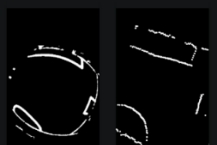
\includegraphics[width=7cm]{gambar/cam_raw2.jpg}
  \caption{Calculated frame.}
  \label{fig:skenariopengujian32}
\end{figure}

The left picture is the line binary image that calculated to get the line coordinates on frame. Extracting the line coordinates on the frame is done by scanning from the center of frame to the edge of frame.  

\begin{algorithm}[htbp]
  \caption{Process Lines on Frame}\label{alg:process_lines}
  \begin{algorithmic}[1]
  \Procedure{ProcessLinesOnFrame}{}
      \State \text{Initialize lines\_on\_frame as an empty vector}
      \For{\text{angle from 0 to 360 with step size 2.5}}
          \State \text{Initialize dist to 0}
          \For{\text{index from 0 to 320}}
              \State $x \gets \text{dist} \times \cos(\text{angle}) + \text{center\_cam\_x}$
              \State $y \gets \text{center\_cam\_y} - \text{dist} \times \sin(\text{angle})$
              \If{\text{frame[y][x] == 255}}
                  \State \text{Push (x, y) to lines\_on\_frame}
              \EndIf
              \State $dist \gets \text{dist} + 1$
          \EndFor
      \EndFor
  \EndProcedure
  \end{algorithmic}
\end{algorithm}

% Dummy
After getting the line coordinates on the frame, the robot will calculate the world coordinates of the line. The formula used to calculate the line's position on the field is as follows:

\begin{equation}
  \begin{aligned}
    dx &= x\_line\_cam - x\_center\_cam \\
    dy &= y\_center\_cam - y\_line\_cam \\
    r\_line\_cam &= \sqrt{dx^2 + dy^2} \\
    \theta\_line\_cam &= \arctan(\frac{dy}{dx}) \\
    index &= \theta\_line\_cam \times r\_max + r\_line\_cam \\ 
    r\_line\_fld &= r\_lookup[index] \\
    \theta\_line\_fld &= \theta\_line\_cam + robot\_\theta - 90 \\
    x\_line &= robot\_x + r\_line\_fld \times \cos(\theta\_line\_fld) \\
    y\_line &= robot\_y + r\_line\_fld \times \sin(\theta\_line\_fld) \\
  \end{aligned}
\end{equation}

After the robot has finished calculating the line's position on the field, the robot will visualize the line on the field. The visualization can be seen on right picture of figure \ref{fig:skenariopengujian32}.


\subsection{Computational Speed Testing Scenario}
\label{sec:analisispengujian}

The test is done by comparing whether the new calibration system is faster than using the old calibration system. The test is done by recording the time after calibration and subtracting it from the time before calibration. So that an estimate of the time it takes for the system to perform the calculation process for calibration can be obtained. The following formula is used to calculate the delay time:

\begin{equation}
  \begin{aligned}
    delay\_time &= time1 - time0 \\ 
  \end{aligned}
\end{equation}

Where $time1$ is the time after calibration and $time0$ is the time before calibration.

\subsection{Computational Speed Testing Evaluation}
\label{sec:analisispengujian}

From the tests that have been carried out, there are 10 iterations that have been done. The following is the data obtained from the test results:

\begin{table}[htpb]
  \caption{Difference in Computational Speed Test Results}
\begin{center}

\begin{tabular}{|c|c|c|}
  \hline
  \rowcolor[HTML]{C0C0C0}
  \textbf{Iteration to-} & \textbf{New Calibration Time} & \textbf{Old Calibration Time} \\
  \hline
  0            & 119 ns                & 176 ns            \\
  1           & 76 ns                & 86 ns            \\
  2           & 25 ns                & 107 ns            \\
  3           & 31 ns                & 90 ns           \\
  4           & 32 ns                & 88 ns           \\
  5           & 36 ns                & 87 ns           \\
  6           & 37 ns                & 88 ns           \\
  7           & 34 ns                & 93 ns           \\
  8           & 37 ns                & 89 ns           \\
  9           & 35 ns                & 90 ns           \\
  \hline
\end{tabular}
\end{center}
\end{table}

From the graph, it can be seen that the new calibration system is 53.2 ns faster than the old calibration system. With an average of 46.2 ns for the new calibration and 99.4 ns for the old calibration. This is because the new calibration system only uses a \emph{Lookup Table} containing camera calibration data. Whereas the old calibration system uses the polynomial regression algorithm which takes longer.



% % Ubah judul dan label berikut sesuai dengan yang diinginkan.
% \section{Kesimpulan}
% \label{sec:kesimpulan}

% % Ubah paragraf-paragraf pada bagian ini sesuai dengan yang diinginkan.

% Dari hasil penelitian yang telah dilakukan, dapat disimpulkan bahwa metode kalibrasi kamera omnivision menggunakan \emph{Machine Learning} lebih baik daripada metode kalibrasi kamera omnivision menggunakan regresi polinomial. Hal ini dapat dilihat dari kemampuan metode kalibrasi kamera omnivision menggunakan \emph{Machine Learning} yang dapat meng-kalibrasi kamera omnivision pada semua arah. Sedangkan metode kalibrasi kamera omnivision menggunakan regresi polinomial hanya dapat meng-kalibrasi kamera omnivision pada satu arah saja. Selain itu, metode kalibrasi kamera omnivision menggunakan \emph{Machine Learning} juga membutuhkan waktu eksekusi yang lebih singkat daripada metode kalibrasi kamera omnivision menggunakan regresi polinomial. 

\section{Conclusion}
\label{sec:conclusion}

From the research that has been done, it can be concluded that the omnivision camera calibration method using Machine Learning is better than the omnivision camera calibration method using polynomial regression. This can be seen from the ability of the omnivision camera calibration method using Machine Learning to calibrate the omnivision camera in all directions. While the omnivision camera calibration method using polynomial regression can only calibrate the omnivision camera in one direction. In addition, the omnivision camera calibration method using Machine Learning also requires a shorter execution time than the omnivision camera calibration method using polynomial regression.
% Acknowledgment jika ada
\section{Acknowledgement}
\label{sec:acknowledgement}

The authors would like to thank the Ministry of Research, Technology, and Higher Education of the Republic of Indonesia for \lipsum[1]

% Menampilkan daftar pustaka dengan format IEEE
\bibliographystyle{IEEEtranN}
\bibliography{pustaka/pustaka.bib}

% Menyeimbangkan bagian akhir di kedua kolom
\balance

\end{document}
